\documentclass{VUMIFInfKursinis}
\usepackage{algorithmicx}
\usepackage{algorithm}
\usepackage{algpseudocode}
\usepackage{amsfonts}
\usepackage{amsmath}
\usepackage{bm}
\usepackage{color}
\usepackage{graphicx}
% \usepackage{hyperref}  % Nuorodų aktyvavimas
\usepackage{url}


% Titulinio aprašas
\university{Vilniaus universitetas}
\faculty{Matematikos ir informatikos fakultetas}
\institute{Informatikos institutas}  % Užkomentavus šią eilutę - institutas neįtraukiamas į titulinį
\department{Informatikos katedra}
\papertype{Operacinių sistemų pirmoji užduotis}
\title{Virtualios ir realios mašinos projektas}
%\titleineng{Modeling of Risk Management Process}
\status{3 kurso 1 grupės studentas}
\author{Dominykas Marma}
% \secondauthor{Vardonis Pavardonis}   % Pridėti antrą autorių
\supervisor{Mantas Grubliauskis}
\date{Vilnius \\ \the\year}

% Nustatymai
% \setmainfont{Palemonas}   % Pakeisti teksto šriftą į Palemonas (turi būti įdiegtas sistemoje)
\bibliography{bibliografija} 

\begin{document}
\maketitle

\tableofcontents

\section{Užduoties aparašymas}

Virtualios mašinos procesoriaus komandos operuoja su duomenimis, esančiais registruose ir ar atmintyje. Yra komandos duomenų persiuntimui iš atminties į registrus ir atvirkščiai, aritmetinės (sudėties, atimties, daugybos, dalybos, palyginimo), sąlyginio ir besąlyginio valdymo perdavimo, įvedimo, išvedimo, darbo su failais (atidarymo, skaitymo, rašymo, uždarymo, sunaikinimo) ir programos pabaigos komandos. Registrai yra tokie: komandų skaitiklis, bent du bendrosios paskirties registrai, požymių registras (požymius formuoja aritmetinės, o į juos reaguoja sąlyginio valdymo perdavimo komandos). Atminties dydis yra 16 blokų po 16 žodžių (žodžio ilgį pasirinkite patys).


Realios mašinos procesorius gali dirbti dviem režimais: vartotojo ir supervizoriaus. Virtualios mašinos atmintis atvaizduojama į vartotojo atmintį naudojant puslapių transliaciją. Yra taimeris, kas tam tikrą laiko intervalą generuojantis pertraukimus. Įvedimui naudojama klaviatūra, išvedimui - ekranas. Yra išorinės atminties įrenginys - kietasis diskas.

Vartotojas, dirbantis su sistema, programas paleidžia interaktyviai, surinkdamas atitinkamą komandą. Laikoma, kad vartotojo programos yra realios mašinos kietajame diske, į kurį jos patalpinamos „išorinėmis", modelio, o ne projektuojamos OS, priemonėmis.

\section{Realios mašinos modelis}

Šiame darbe bus modeliuojama reali mašina, kuri turi vieną procesorių. Jos modelis yra pateikiamas \ref{img:reali_masina} paveiksliuke. Tolesnėse sekcijose bus plačiau aprašoma kiekviena šios mašinos dalis

\begin{figure}[H]
	\centering	
	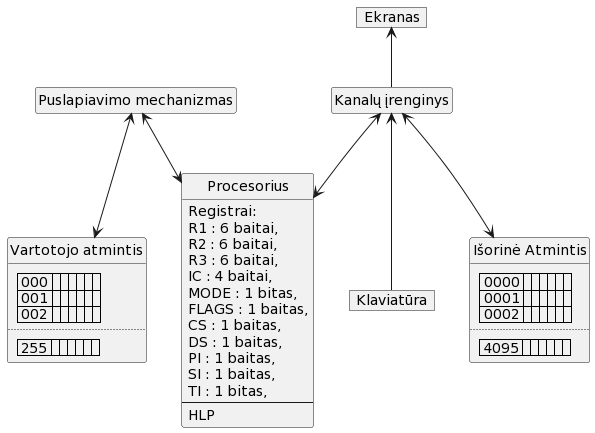
\includegraphics[scale=0.65]{img/reali_masina}
	\caption{Realios mašinos modelis}   % Antraštė įterpiama po paveikslėlio
	\label{img:reali_masina}
\end{figure}

\subsection{Procesorius}

Procesorius turi registrus:

\begin{itemize}
	\item IC - komandų skaitiklis - 4 baitai.
	\item R1, R2, R3 - bendrosios paskirties registrai iš 6 baitų (vienas žodis).
	\item CS - kodo segmento registras, 1 baitas.
	\item DS - duomenų segmento registras, 1 baitas.
	\item MODE - 1 bito registras, kuris nurodo procesoriaus darbo rėžimą (0 - vartotojas, 1 - supervizorius)
	\item FLAGS - požymių  registras, susidedantis iš šių 2 bitų (nuo didžiausio iki mažiausio): 
	\begin{itemize}
		\item ZF - yra 1, jei aritmetinės ar palyginimo operacijos rezultatas yra 0, o kitu atveju išvalomas.
		\item SF - nustatomas 1, jei aritmetinės operacijos rezultatas yra teigiamas, o priešingu atveju - 0.
	\end{itemize}
	\item PTR - puslapiavimo registras - 2 baitai
	\item PI - 1 bito programinių pertraukimų registras.
	\item TI - 1 bito laikrodžio pertraukimas registras.
	\item SI - 1 bito sisteminių pertraukimų registras.
\end{itemize}

Be registrų procesorius dar turi Aukšto lygio kalbos procesorių - HLP. Jis atsakingas už komandų apdorojimą.

\subsection{Vartotojo atmintis}

Mašinos atminties dydis yra 16 blokų po 16 žodžių. Vieno žodžio ilgis yra 6 baitai.

\subsubsection{Puslapiavimas}

Norint virtualios mašinos blokų numerius paversti į realios mašinos blokų numerius yra taikomas puslapiavimo mechanizmas. Tam tikslui, kuriant virtualią mašiną, yra išskiriamas dar vienas blokas, kuriame saugama lentelė, atliekanti pervertimą.

Kai PTR reikšmė yra $a_0a_1$, kur $a_0, a_1$ yra baitai, tai $a_0$ rodo puslapiavimo lentelės bloko numerį, o $a_1$ - lentelės pradžios adresą tame bloke (abu šešioliktainiu formatu).

Virtualaus adreso $x_0x_1$ realus adresas = $16 * [(16 * a_0 + a_1) + x_0] + x_1$.

\subsection{Taimerio mechanizmas}
Realioje mašinoje yra taimeris. Jis skirtas tam, kad viena užduotis nebūtų vykdoma daugiau nei 20 laiko momentų. Tam tikslui po kiekvienos operacijos yra sumažina TI reikšmė. Skirtingos operacijos užtrunka skirtingą laiko skaičių: išvedimo į kanalų įrenginį ar įvedimo į jį užima 5 laiko vienetus, o visos kitos - 1. Kai TI reikšmė pasiekia 0 yra sugeneruojamas taimerio pertraukimas ir valdymas perduodamas supervizoriui.

\subsection{Kanalų įrenginys}

Realioje mašinoje yra įvedimo įrenginys - klaviatūra ir išvedimo įrenginys - ekranas. Jie su procesorium komunikuoja per kanalų įrenginį. Įvydžius apsikeitimo komandą EXCHGE yra perkeliamas vienas baitas. Tam, kad būtų specifikuota, tai, kas bus perkeliama yra naudojami šie kanalų įrenginio registrai:

\begin{itemize}
	\item SB - 1 baito registras, kuriame saugomas takelio, iš kurio bus kopijuojama numeris.
	\item SW - 1 baito registras, kuriame saugoma žodžio iš kurio bus kopijuojama numeris.
	\item DB - 1 baito registras, kuriame saugas takelio, į kurį bus kopijuojama
	\item DW - 1 baito registras, kuriame saugoma žodžio į kurį  bus kopijuojama numeris.
	\item ST - 1 baito registras, kuriame nurodytas tipas objekto, kuris bus kopijuotas. 
	\begin{enumerate}
		\item Procesoriaus atmintis
		\item Išorinė atmintis
		\item Klaviatūra
	\end{enumerate}
	\item DT - 1 baito registras, kuriame nurodytas tipas objekto, į kurį bus kopijuojama
	\begin{enumerate}
		\item Procesoriaus atmintis
		\item Išorinė atmintis
		\item Ekranas
	\end{enumerate}
\end{itemize}

\subsection{Išorinė Atmintis}

Išorinė atmints yra realizuojama kietuoju disku. Jame yra 256 blokai po 16 žodžių.

Komunikacija su išorine atmintimi yra vykdoma per kanalų įrenginį.

\subsection{Klaviatūra}

Kiekvienas klaviatūros mygtuko paspaudimas generuoja sisteminius pertraukimus, t.y. nustato registro SI reikšmę į 1. 

Reali mašina įsimena paskutinį simbolį ir jį ligi simbolis yra perskaitomas. Kai tai nutinka vietoje simbolio yra įrašoma reikšmė 0. Jei tokiu metu yra bandoma skaityti, tai laikoma, kad tai nepavyko.

\subsection{Ekranas}

Į ekraną galima išvesti vieną žodį. Tam programa turi perkelti reikšmę į R1 ir iškviesti sisteminius pertraukimą

\section{Virtualios mašinos modelis}

Virtuali mašina - operacinės sistemos konstruktas, kurio pagalba kiekvienos programos veikimas yra izoliajamos nuo visų kitų, o darbui su bendrais įrenginiais pasitelkiama operacinė sistemą. Reali mašina paleidžia virtualią mašiną, o ši vykdo komandas. Šios mašinos modelis yra pateikiamas \ref{img:virtuali_masina} paveiksliuke.

\begin{figure}[H]
	\centering	
	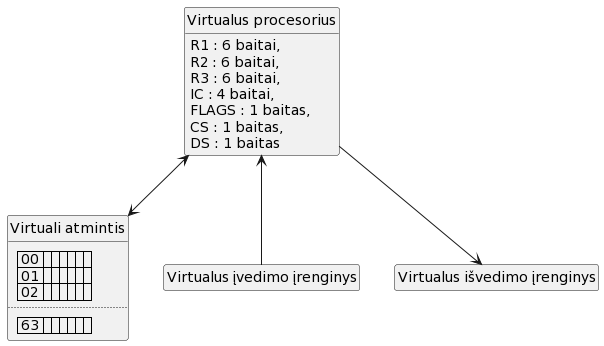
\includegraphics[scale=0.65]{img/virtuali_masina}
	\caption{Virtualios mašinos modelis}   % Antraštė įterpiama po paveikslėlio
	\label{img:virtuali_masina}
\end{figure}

\subsection{Registrai}

Virtuali mašina turi priėjimą tik prie šių realios mašinos registrų:

\begin{itemize}
	\item R1, R2, R3 (bendros paskirties registrai)
	\item CS (kodo segmento registras)
	\item DS (duomenų segmento registras)
	\item FLAGS (požymių registras)
	\item IC (programos skaitiklis)
\end{itemize}

\subsection{Atmintis}

Virtuali mašina turi priėjimą prie 4 blokų. Virtuali mašina gauna blokų virtualius numerius. Dėl to kiekviena virtuali mašina mato, kad jos blokai yra pirmi keturi - 0, 1, 2, 3.

\subsection{Komandos}

Visos komandos yra aprašomos vienu žodžiu - 6 baitais. Visose komandose simbolis * reiškia, kad šis baitas nėra naudojamas.

\subsubsection{Aritmetinės}
Šiose operacijose $x, y \in \{1, 2, 3\}$, o $m \in \{0, 1\}$
\begin{itemize}
	\item ADDmxy - jei m = 0, tai operacija sudeda skaičius esančius registruose Rx, Ry ir rezultatą patalpina į R1.
	\item SUBmxy - jei m = 0, tai operacija atima iš skaičiaus esančio registre Rx, skaičių iš registro Ry ir rezultatą patalpina į R1. Jei m=1, tai operaciją atlieka su registru Rx ir konstanta y.
	\item MULmxy - jei m = 0, tai operacija sudaugina skaičius esančius registruose Rx, Ry ir rezultatą patalpina į R1. Jei m=1, tai operaciją atlieka su registru Rx ir konstanta y.
	\item DIVmxy - jei m = 0, tai operacija padalina skaičių esantį registre Rx, iš skaičiaus esančio registre Ry ir rezultatą patalpina į R1. Jei m=1, tai operaciją atlieka su registru Rx ir konstanta y.
	\item CMPmxy - jei m = 0, tai operacija palygina skaičius esančius registruose Rx ir Ry bei pagal Rx-Ry reikšmę nustato registro FLAGS reikšmę. Jei m=1, tai operaciją atlieka su registru Rx ir konstanta y.
\end{itemize}

Po kiekvienos aritmetinės operacijos procesorius padina IC reikšmę. Taip pat po kiekvienos aritmetinės operacijos pagal rezultatą (o palyginimo atveju - lyginamųjų skaičių skirtumą) yra nustatomos registro FLAGS reikšmės.

\begin{itemize}
	\item Jei rezultatas yra 0, tai nustatomas ZF=1, kitu atveju ZF = 0.
	\item SF reikšmė yra nustatoma rezultato didžiausio bito reikšmei.
\end{itemize}

\subsubsection{Duomenų judėjimo}
\begin{itemize}
	\item MVmxy* - Perkelia duomenis. m reikšmė nurodo perkelimo režimą. x ir y specifikuoja vietas, kur juda duomenys. Po šios komandos yra padidinama IC reikšmė.
	\begin{enumerate}
		\item m = 1. Šiuo atveju perkėlimas yra iš registro į registrą. x nurodo pirmo registro (šaltinio) numerį, y - tikslo.
		\item m = 2. Šiuo atveju perkėlimas yra iš registro R1 į atmintį. Atminties vieta yra gaunama pagal formulę $10 \cdot x + y$.
		\item m = 3. Šiuo atveju perkėlimas yra iš atminties į registrą R1. Atminties vieta yra gaunama pagal formulę $10 \cdot x + y$.
	\end{enumerate}
\end{itemize}

\subsubsection{Valdymo}
Norint tinkamai naudotis perėjimais, prieš juos reikia panaudoti CMP operaciją. 
\begin{itemize}
	\item JMPxyz - besąlyginis perėjimas. $x, y, z \in \{1, 2, \cdots 9 \}$. IC := 100*x + 10 * y + z.
	\item JExyz* - pereiti, jeigu lygu. $x, y, z \in \{1, 2, \cdots 9 \}$. Jei ZF=1, tai IC := 100*x + 10 * y + z, kitu atveju IC := IC + 1.
	\item JNExyz* - pereiti, jei nelygu. $x, y, z \in \{1, 2, \cdots 9 \}$. Jei ZF=0, tai IC := 100*x + 10 * y + z, kitu atveju IC := IC + 1.
	\item JLxyz* - pereiti, jeigu mažiau. $x, y, z \in \{1, 2, \cdots 9 \}$. Jei SF=1, tai IC := 100*x + 10 * y + z, kitu atveju IC := IC + 1.
	\item JLExyz* - pereiti, jeigu mažiau arba lygu. $x, y, z \in \{1, 2, \cdots 9 \}$. Jei ZF=1 arba SF=1, tai IC := 100*x + 10 * y + z, kitu atveju IC := IC + 1.
	\item JGxyz* - pereiti, jeigu daugiau. $x, y, z \in \{1, 2, \cdots 9 \}$. Jei SF=0, tai IC := 100*x + 10 * y + z, kitu atveju IC := IC + 1.
	\item JGExyz* - pereiti jeigu daugiau arba lygu. $x, y, z \in \{1, 2, \cdots 9 \}$. Jei ZF=1 arba SF=0, tai IC := 100*x + 10 * y + z, kitu atveju IC := IC + 1.
\end{itemize}

Po valdymo komandų registro FLAGS reikšmė nėra keičiama.

\subsubsection{Darbas su failais}
Darbo su failais metu yra naudojamos simbolių eilutės. Tai baitų seka, kurios pabaigoje yra žodis 000000. Visos šios operacijos iškviečia programinius pertraukimus, o procesoriui reikalinga informacija apie komandos paskirtį yra gauname per komandos pavadinimą.
\begin{itemize}
	\item OPENF* - atidaro failą, kurio pavadinimas yra simbolių eilutė, kurios pradžios adresas yra R1 reikšmė. Operacijos pabaigoje į R2 yra įrašomas failo numeris. Jeigu failas yra nerandamas - nustato SI=1.
	\item CLOSEF - uždaro failą, kurio numeris yra įrašytas  R2. Jeigu norimas failas nėra rastas, ar jau buvo uždarytas yra nustatoma R1 = 0, kitu atveju R1 bus uždaryto failo numeris.
	\item WRITEF - parašo simbolį iš R1 į failą, kurio numeris yra R2.
	\item READ** - kai R2 yra nuskaitomo failo numeris, perskaito simbolį iš failo ir jo reikšmę įrašo į R1.
	\item DELETF - sunaikiną failą, kurio numeris nurodomas R2 reikmšmėje.
\end{itemize}

Po kiekvienos iš šių komandų procesorius padidina registro IC reikšmę ir išvalo FLAGS registrą.

\subsubsection{Įvedimas ir išvedimas}
Įvedimo ir išvedimo komandos, kaip ir darbo su failais komandos, iškviečia sisteminį pertraukimą.
\begin{itemize}
	\item INTER1 - išveda registro R1 reikšmę į ekraną.
	\item INTER2 - perskaito simbolį įvestą iš klaviatūros bei reikšmę patalpina į R1. Iki kol simbolis yra įvedamas, programa užsiblokuoja. Jeigu nuskaityti nepavyko, tai gauname reikšmė R1=0.
\end{itemize}

\subsubsection{Programos pabaigos}
\begin{itemize}
	\item HALT** - baigia programos darbą.
\end{itemize}

\subsubsection{Neaptartos situacijos}

Jeigu programos vykdymo metu yra sutinkama komanda, kurios procesorius nesugeba apdoroti, tai jokia programa nėra vykdoma ir padidinama IC reikšmė.

Jei programos vykdymo metu IC reikšmė viršija $63_{10}$ (programos žodžių skaičius), tai programa yra nutraukiama.

\subsection{Programos struktūra}

Maksimalus programos dydis yra 64 žodžiai.

Programos pradžią žymi žodis \$START. Po jo yra programos pavadinimas, o žymė ------ (šeši '-' ženklai) - pavadinimo pabaigą. 

Tarp šių žodžių yra rašomos programos komandos. Jos užima vieta kode nuo programos pradžios. 

Nuo $10_{10}$ žodžio yra kodo segentas. Programos pradžioje nustatoma IC = $10_{10}$. Tam, kad kode nereikėtų vesti tuščių simbolių kodo segmentas žymimas .CODES žyme.

Nuo $40_{10}$ žodžio yra duomenų segmento vieta. Visi nuo šio žodžio sekantys žodžiai yra perkeliami į programą, o jei jų iki pabaigos žymės yra mažiau - programa užpildoma nuliais.
Tam, kad kode nereikėtų vesti tuščių simbolių duomenų segmentas žymimas .DATAS žyme.

Programos pabaiga žymi žodis \$FINSH. 

\subsection{Išorinio disko pavyzdys}

\begin{verbatim}
	
$START
ciklas
------
.CODES
JMP010
.DATAS
$FINSH
$START
sudeti
------
.CODES
INTER2
MV112*
INTER2
ADD012
INTER1
.DATAS
$FINISH

	
\end{verbatim}


\subsection{Virtuali mašina operacinės sistemos kontekste}

Operacinė sistema paleidžia virtualią mašiną kiekvienai programai. Jei operacinė sistema yra multiprograminė, tai joje vienu metu veikia tik viena programa, bet vykdomoji programa nuolatos keičiasi.

Virtualias mašinas kuria operacinė sistemą. Jos yra sukuriamos, kai vartotojas įveda programą LOAD prg, kur prg yra programos pavadinimas kietąjame diske.

\printbibliography[heading=bibintoc] % Literatūros šaltiniai aprašomi
\appendix  % Priedai

\end{document}
